% Seminarul 0: Introducere
% Statistica piețelor financiare -- Program de licență, Academia de Studii Economice din București
% GENERAT de latex/build_seminar0.py -- modificați generatorul, nu acest fișier.
% Implicit versiunea pentru studenți; versiunea profesorului este wrapper-ul *_solutions.tex.
\makeatletter\@ifundefined{ifsolutions}{\expandafter\newif\csname ifsolutions\endcsname}{}\makeatother

\newcommand{\coursename}{Statistica piețelor financiare}
\def\sfmlang{ro}
% Preambul comun SFM -- Statistica piețelor financiare / Statistics of Financial Markets (Beamer, 16:9)
% Același design ca MFM. Înainte de % Preambul comun SFM -- Statistica piețelor financiare / Statistics of Financial Markets (Beamer, 16:9)
% Același design ca MFM. Înainte de % Preambul comun SFM -- Statistica piețelor financiare / Statistics of Financial Markets (Beamer, 16:9)
% Același design ca MFM. Înainte de \input{../../latex/preamble} se definește
%   \newcommand{\coursename}{Statistics of Financial Markets}      (EN)
%   \newcommand{\coursename}{Statistica piețelor financiare}       (RO)  și  \def\sfmlang{ro}
% Fișierele .tex se află în EN/Courses, EN/Seminars, RO/Cursuri, RO/Seminarii (două niveluri sub rădăcină).
% Deck-urile sînt generate de latex/build_chapterN.py / build_seminarN.py (vezi latex/sfm_build.py).

\documentclass[9pt, aspectratio=169, t]{beamer}
\providecommand{\coursename}{Statistics of Financial Markets}

% Ensure content fits on slides
\setbeamersize{text margin left=8mm, text margin right=8mm}

%=============================================================================
% THEME AND STYLE CONFIGURATION
%=============================================================================
\usetheme{default}
% Using default theme for clean header/footer control

% Color Palette (matching Redispatch PDF)
\definecolor{MainBlue}{RGB}{26, 58, 110}
\definecolor{AccentBlue}{RGB}{26, 58, 110}
\definecolor{IDAred}{RGB}{205, 0, 0}
\definecolor{DarkGray}{RGB}{51, 51, 51}
\definecolor{MediumGray}{RGB}{128, 128, 128}
\definecolor{LightGray}{RGB}{248, 248, 248}
\definecolor{VeryLightGray}{RGB}{235, 235, 235}
\definecolor{KeynoteGray}{RGB}{218, 218, 218}
\definecolor{SectionGray}{RGB}{120, 120, 120}
\definecolor{FooterGray}{RGB}{100, 100, 100}
\definecolor{Crimson}{RGB}{220, 53, 69}
\definecolor{Forest}{RGB}{46, 125, 50}
\definecolor{Amber}{RGB}{181, 133, 63}
\definecolor{Orange}{RGB}{230, 126, 34}
\definecolor{Purple}{RGB}{142, 68, 173}

% Gradient background (exact Keynote 315° gradient: white to RGB 218,218,218)
\setbeamertemplate{background}{%
    \begin{tikzpicture}[remember picture, overlay]
        \shade[shading=axis, shading angle=315,
        top color=white, bottom color=KeynoteGray]
        (current page.south west) rectangle (current page.north east);
    \end{tikzpicture}%
}
% Fallback solid color for compatibility
\setbeamercolor{background canvas}{bg=}

\setbeamercolor{palette primary}{bg=MainBlue, fg=white}
\setbeamercolor{palette secondary}{bg=MainBlue!85, fg=white}
\setbeamercolor{palette tertiary}{bg=MainBlue!70, fg=white}
\setbeamercolor{structure}{fg=MainBlue}
\setbeamercolor{title}{fg=IDAred}
\setbeamercolor{frametitle}{fg=IDAred, bg=}
\setbeamercolor{block title}{bg=MainBlue, fg=white}
\setbeamercolor{block body}{bg=VeryLightGray, fg=DarkGray}
\setbeamercolor{block title alerted}{bg=Crimson, fg=white}
\setbeamercolor{block body alerted}{bg=Crimson!8, fg=DarkGray}
\setbeamercolor{block title example}{bg=Forest, fg=white}
\setbeamercolor{block body example}{bg=Forest!8, fg=DarkGray}
\setbeamercolor{item}{fg=MainBlue}

% Footer colors (override Madrid theme blue)
\setbeamercolor{author in head/foot}{fg=FooterGray, bg=}
\setbeamercolor{title in head/foot}{fg=FooterGray, bg=}
\setbeamercolor{date in head/foot}{fg=FooterGray, bg=}
\setbeamercolor{section in head/foot}{fg=FooterGray, bg=}
\setbeamercolor{subsection in head/foot}{fg=FooterGray, bg=}

% Bullet styles (apply everywhere including blocks)
\setbeamertemplate{itemize item}{\color{MainBlue}$\boxdot$}
\setbeamertemplate{itemize subitem}{\color{MainBlue}$\blacktriangleright$}
\setbeamertemplate{itemize subsubitem}{\color{MainBlue}\tiny$\bullet$}
\setbeamertemplate{itemize/enumerate body begin}{\normalsize}
\setbeamertemplate{itemize/enumerate subbody begin}{\normalsize}

% Item spacing - compact style
\setlength{\leftmargini}{10pt}       % Level 1: minimal indent
\setlength{\leftmarginii}{10pt}      % Level 2: minimal additional indent
% Compact list spacing (zero extra space before/after lists in blocks)
\makeatletter
\def\@listi{\leftmargin\leftmargini \topsep 0pt \parsep 0pt \itemsep 0pt}
\def\@listii{\leftmargin\leftmarginii \topsep 0pt \parsep 0pt \itemsep 0pt}
\makeatother

\setbeamertemplate{navigation symbols}{}

%=============================================================================
% CUSTOM HEADLINE
%=============================================================================
\setbeamertemplate{headline}{%
    \vskip10pt%
    \hbox to \paperwidth{%
        \hskip0.5cm%
        {\small\color{FooterGray}\renewcommand{\hyperlink}[2]{##2}\insertsectionhead}%
        \hfill%
        \textcolor{FooterGray}{\small\insertframenumber}%
        \hskip0.5cm%
    }%
    \vskip4pt%
    {\color{FooterGray}\hrule height 0.4pt}%
}

%=============================================================================
% CUSTOM FOOTER
%=============================================================================
\usepackage{fontawesome5}

\setbeamertemplate{footline}{%
    {\color{FooterGray}\hrule height 0.4pt}%
    \vskip4pt%
    \hbox to \paperwidth{%
        \hskip0.5cm%
        \textcolor{FooterGray}{\small\coursename}%
        \hfill%
        \raisebox{-0.1em}{%
            \begin{tikzpicture}[x=0.08em, y=0.08em, line width=0.4pt]
                \draw[FooterGray] (0,3) -- (1,4) -- (2,3.5) -- (3,5) -- (4,4) -- (5,6) -- (6,5.5) -- (7,4) -- (8,5) -- (9,7) -- (10,6) -- (11,5) -- (12,6.5) -- (13,8) -- (14,7) -- (15,6) -- (16,7.5) -- (17,9) -- (18,8) -- (19,7) -- (20,8.5) -- (21,10) -- (22,9) -- (23,8) -- (24,9.5);
            \end{tikzpicture}%
        }%
        \hskip0.5cm%
    }%
    \vskip6pt%
}

%=============================================================================
% PACKAGES
%=============================================================================
\usepackage[utf8]{inputenc}
\DeclareUnicodeCharacter{03B1}{\ensuremath{\alpha}}
\usepackage[T1]{fontenc}
\usepackage{amsmath, amssymb, amsthm}
\usepackage{mathtools}
\usepackage{bm}
\usepackage{tikz}
\usetikzlibrary{arrows.meta, positioning, shapes, calc, decorations.pathreplacing, shadings}
\usepackage{booktabs}
\usepackage{multirow}
\usepackage{array}
\usepackage{graphicx}
\usepackage{hyperref}
\usepackage{colortbl}
\usepackage{listings}
\lstset{language=Python, basicstyle=\ttfamily\scriptsize, keywordstyle=\color{MainBlue}\bfseries,
  commentstyle=\color{Forest}, stringstyle=\color{Crimson}, breaklines=true,
  frame=none, backgroundcolor=\color{VeryLightGray}, xleftmargin=2mm}
\hypersetup{colorlinks=true, linkcolor=MainBlue, urlcolor=MainBlue}
\graphicspath{{../../logos/}{../../charts/}{../../photos/}}
\usepackage{xcolor}
\hfuzz=2pt  % Suppress tiny overfull warnings (<2pt)
\vfuzz=2pt  % Suppress tiny vertical overfull warnings (<2pt)

%=============================================================================
% QUANTLET COMMANDS
%   \quantlet{<displayed name>}{<url>}       (generic, compatible with the older SFM decks)
%   \sfmquantlet{Ch_05}{SFM_ch5_garch}       -> https://github.com/danpele/SFM/tree/main/Quantlets/Ch_05/SFM_ch5_garch
%   \qlurl{<folder>} is defined per chapter by the generator (Quantlets/Ch_NN/<folder>)
%=============================================================================
\newcommand{\sfmrepo}{https://github.com/danpele/SFM}
\newcommand{\sfmqlbase}{https://github.com/danpele/SFM/tree/main/Quantlets}
\newcommand{\quantlet}[2]{%
    \hfill\href{#2}{%
        \raisebox{-0.15em}{
\includegraphics[height=0.7em]{ql_logo.png}}%
        \textcolor{MainBlue}{\tiny\ #1}%
    }%
}
\newcommand{\sfmquantlet}[2]{\quantlet{\detokenize{#2}}{\sfmqlbase/#1/#2}}

%=============================================================================
% NOTEBOOKS (Google Colab)
%   \colaburl{notebooks/EN/chapter5_seminar_notebook.ipynb} -> the Colab link of a file in the SFM repo
%   \nb: the chapter notebook (each seminar deck redefines it with \renewcommand)
%=============================================================================
\newcommand{\colaburl}[1]{https://colab.research.google.com/github/danpele/SFM/blob/main/#1}
\newcommand{\nb}{https://colab.research.google.com/github/danpele/SFM/tree/main/notebooks/EN}
\newcommand{\nbname}{notebooks/EN}

%=============================================================================
% SLIDE HELPERS (used by the generators; the same as in MFM)
%=============================================================================
% local font size for list bodies (the preamble forces \normalsize)
\newcommand{\itemsize}[1]{\setbeamertemplate{itemize/enumerate body begin}{#1}\setbeamertemplate{itemize/enumerate subbody begin}{#1}}
\newcommand{\intitle}[1]{{\hypersetup{urlcolor=white}#1}}   % white links inside coloured title bars
\newcommand{\imgcap}[1]{{\scriptsize #1}\\[0.5mm]}          % caption under a photo
\newcommand{\imgcredit}[2]{{\tiny\color{FooterGray}\href{#1}{#2}}}   % image credit: source URL, author/licence
\newcommand{\aiprompt}[1]{{\ttfamily\color{MainBlue}#1}}     % a prompt to an AI assistant

%=============================================================================
% SEMINARS: student version by default; the instructor wrapper *_solutions.tex sets \solutionstrue
%=============================================================================
\makeatletter\@ifundefined{ifsolutions}{\expandafter\newif\csname ifsolutions\endcsname}{}\makeatother
\newcommand{\solonly}[1]{\ifsolutions #1\fi}
\newcommand{\propsub}{\ifsolutions\else\framesubtitle{\ifdefined\sfmlang Rezolvarea se discută la seminar\else Solution discussed in class\fi}\fi}

%=============================================================================
% APPENDIX AND CHAPTER LINKS (latex/appendix_links.py writes the calls; it also re-declares these
% macros before \begin{document}, so the decks compile with or without this preamble block)
%=============================================================================
\providecommand{\sfmapplink}[3]{\hypertarget{#2}{}\hyperlink{#1}{\beamergotobutton{#3}}}
\providecommand{\sfmappback}[2]{\begin{tikzpicture}[remember picture,overlay]\node[anchor=south east] at ([xshift=-3mm,yshift=7mm]current page.south east){\hyperlink{#1}{\beamerreturnbutton{#2}}};\end{tikzpicture}}
\providecommand{\sfmchlink}[2]{\href{#1}{#2}}
\providecommand{\sfmchlinkt}[2]{\href{#1}{\usebeamercolor[fg]{frametitle}#2}}

%=============================================================================
% QUANTINAR COMMAND: link către un curs Quantinar (subiecte avansate)
%=============================================================================
\newcommand{\quantinar}[2]{%
    \href{#2}{%
        \raisebox{-0.15em}{
\includegraphics[height=0.8em]{qr_logo.png}}%
        \textcolor{MainBlue}{\scriptsize\ #1}%
    }%
}

%=============================================================================
% CUSTOM TITLE PAGE
%=============================================================================
\defbeamertemplate*{title page}{hybrid}[1][]
{
    \vspace{0.2cm}
    % Logos row - top header (with clickable links)
    \begin{center}
        \href{https://www.ase.ro}{
\includegraphics[height=1.0cm]{ase_logo.png}}\hspace{0.3cm}%
        \href{https://theida.net}{
\includegraphics[height=1.0cm]{ida_logo.png}}\hspace{0.3cm}%
        \href{https://blockchain-research-center.com}{
\includegraphics[height=1.0cm]{brc_logo.png}}\hspace{0.3cm}%
        \href{https://www.ai4efin.ase.ro}{
\includegraphics[height=1.0cm]{ai4efin_logo.png}}\hspace{0.3cm}%
        \href{https://ipe.ro/new}{
\includegraphics[height=1.0cm]{acad_logo.png}}\hspace{0.3cm}%
        \href{https://www.digital-finance-msca.com}{
\includegraphics[height=1.0cm]{msca_logo.png}}%
    \end{center}

    \vspace{0.6cm}

    % Main title with Q logos on sides (with clickable links)
    \begin{center}
        \begin{minipage}{0.1\textwidth}
            \centering
            \href{https://quantlet.com}{
\includegraphics[height=1.1cm]{ql_logo.png}}
        \end{minipage}%
        \begin{minipage}{0.78\textwidth}
            \centering
            {\LARGE\bfseries\usebeamercolor[fg]{title}\inserttitle}

            \vspace{0.3cm}

            {\usebeamerfont{subtitle}\usebeamercolor[fg]{title}\insertsubtitle}
        \end{minipage}%
        \begin{minipage}{0.1\textwidth}
            \centering
            \href{https://quantinar.com}{
\includegraphics[height=1.1cm]{qr_logo.png}}
        \end{minipage}
    \end{center}

    \vspace{0.6cm}

    % Authors (left aligned)
    \hspace{0.5cm}{\usebeamerfont{author}\insertauthor}

    \vspace{0.3cm}

    % Institute/Affiliations (left aligned)
    \hspace{0.5cm}\begin{minipage}[t]{0.9\textwidth}
        \raggedright\small\insertinstitute
    \end{minipage}
}

%=============================================================================
% THEOREM ENVIRONMENTS
%=============================================================================
\theoremstyle{definition}
\setbeamertemplate{theorems}[numbered]
\ifdefined\sfmlang
\newtheorem{defn}{Definiție}
\newtheorem{thm}{Teoremă}
\newtheorem{prop}{Propoziție}
\newtheorem{rmk}{Observație}
\else
\newtheorem{defn}{Definition}
\newtheorem{thm}{Theorem}
\newtheorem{prop}{Proposition}
\newtheorem{rmk}{Remark}
\fi

%=============================================================================
% CENTRED MINIPAGE (no extra vertical space)
%=============================================================================
\newenvironment{cminipage}[1]{%
    \par\noindent\hfill\begin{minipage}{#1}\ignorespaces
}{%
    \end{minipage}\hfill\null\par
}

%=============================================================================
% CUSTOM COMMANDS
%=============================================================================
\newcommand{\E}{\mathbb{E}}
\newcommand{\Var}{\text{Var}}
\newcommand{\Cov}{\text{Cov}}
\newcommand{\Corr}{\text{Corr}}
\newcommand{\R}{\mathbb{R}}
\newcommand{\N}{\mathbb{N}}
\newcommand{\Z}{\mathbb{Z}}
\newcommand{\B}{\mathbf{B}}
\newcommand{\imark}{\textcolor{MainBlue}{\textbullet}}
\newcommand{\RMSE}{\text{RMSE}}
\newcommand{\MAE}{\text{MAE}}
\newcommand{\MAPE}{\text{MAPE}}

 se definește
%   \newcommand{\coursename}{Statistics of Financial Markets}      (EN)
%   \newcommand{\coursename}{Statistica piețelor financiare}       (RO)  și  \def\sfmlang{ro}
% Fișierele .tex se află în EN/Courses, EN/Seminars, RO/Cursuri, RO/Seminarii (două niveluri sub rădăcină).
% Deck-urile sînt generate de latex/build_chapterN.py / build_seminarN.py (vezi latex/sfm_build.py).

\documentclass[9pt, aspectratio=169, t]{beamer}
\providecommand{\coursename}{Statistics of Financial Markets}

% Ensure content fits on slides
\setbeamersize{text margin left=8mm, text margin right=8mm}

%=============================================================================
% THEME AND STYLE CONFIGURATION
%=============================================================================
\usetheme{default}
% Using default theme for clean header/footer control

% Color Palette (matching Redispatch PDF)
\definecolor{MainBlue}{RGB}{26, 58, 110}
\definecolor{AccentBlue}{RGB}{26, 58, 110}
\definecolor{IDAred}{RGB}{205, 0, 0}
\definecolor{DarkGray}{RGB}{51, 51, 51}
\definecolor{MediumGray}{RGB}{128, 128, 128}
\definecolor{LightGray}{RGB}{248, 248, 248}
\definecolor{VeryLightGray}{RGB}{235, 235, 235}
\definecolor{KeynoteGray}{RGB}{218, 218, 218}
\definecolor{SectionGray}{RGB}{120, 120, 120}
\definecolor{FooterGray}{RGB}{100, 100, 100}
\definecolor{Crimson}{RGB}{220, 53, 69}
\definecolor{Forest}{RGB}{46, 125, 50}
\definecolor{Amber}{RGB}{181, 133, 63}
\definecolor{Orange}{RGB}{230, 126, 34}
\definecolor{Purple}{RGB}{142, 68, 173}

% Gradient background (exact Keynote 315° gradient: white to RGB 218,218,218)
\setbeamertemplate{background}{%
    \begin{tikzpicture}[remember picture, overlay]
        \shade[shading=axis, shading angle=315,
        top color=white, bottom color=KeynoteGray]
        (current page.south west) rectangle (current page.north east);
    \end{tikzpicture}%
}
% Fallback solid color for compatibility
\setbeamercolor{background canvas}{bg=}

\setbeamercolor{palette primary}{bg=MainBlue, fg=white}
\setbeamercolor{palette secondary}{bg=MainBlue!85, fg=white}
\setbeamercolor{palette tertiary}{bg=MainBlue!70, fg=white}
\setbeamercolor{structure}{fg=MainBlue}
\setbeamercolor{title}{fg=IDAred}
\setbeamercolor{frametitle}{fg=IDAred, bg=}
\setbeamercolor{block title}{bg=MainBlue, fg=white}
\setbeamercolor{block body}{bg=VeryLightGray, fg=DarkGray}
\setbeamercolor{block title alerted}{bg=Crimson, fg=white}
\setbeamercolor{block body alerted}{bg=Crimson!8, fg=DarkGray}
\setbeamercolor{block title example}{bg=Forest, fg=white}
\setbeamercolor{block body example}{bg=Forest!8, fg=DarkGray}
\setbeamercolor{item}{fg=MainBlue}

% Footer colors (override Madrid theme blue)
\setbeamercolor{author in head/foot}{fg=FooterGray, bg=}
\setbeamercolor{title in head/foot}{fg=FooterGray, bg=}
\setbeamercolor{date in head/foot}{fg=FooterGray, bg=}
\setbeamercolor{section in head/foot}{fg=FooterGray, bg=}
\setbeamercolor{subsection in head/foot}{fg=FooterGray, bg=}

% Bullet styles (apply everywhere including blocks)
\setbeamertemplate{itemize item}{\color{MainBlue}$\boxdot$}
\setbeamertemplate{itemize subitem}{\color{MainBlue}$\blacktriangleright$}
\setbeamertemplate{itemize subsubitem}{\color{MainBlue}\tiny$\bullet$}
\setbeamertemplate{itemize/enumerate body begin}{\normalsize}
\setbeamertemplate{itemize/enumerate subbody begin}{\normalsize}

% Item spacing - compact style
\setlength{\leftmargini}{10pt}       % Level 1: minimal indent
\setlength{\leftmarginii}{10pt}      % Level 2: minimal additional indent
% Compact list spacing (zero extra space before/after lists in blocks)
\makeatletter
\def\@listi{\leftmargin\leftmargini \topsep 0pt \parsep 0pt \itemsep 0pt}
\def\@listii{\leftmargin\leftmarginii \topsep 0pt \parsep 0pt \itemsep 0pt}
\makeatother

\setbeamertemplate{navigation symbols}{}

%=============================================================================
% CUSTOM HEADLINE
%=============================================================================
\setbeamertemplate{headline}{%
    \vskip10pt%
    \hbox to \paperwidth{%
        \hskip0.5cm%
        {\small\color{FooterGray}\renewcommand{\hyperlink}[2]{##2}\insertsectionhead}%
        \hfill%
        \textcolor{FooterGray}{\small\insertframenumber}%
        \hskip0.5cm%
    }%
    \vskip4pt%
    {\color{FooterGray}\hrule height 0.4pt}%
}

%=============================================================================
% CUSTOM FOOTER
%=============================================================================
\usepackage{fontawesome5}

\setbeamertemplate{footline}{%
    {\color{FooterGray}\hrule height 0.4pt}%
    \vskip4pt%
    \hbox to \paperwidth{%
        \hskip0.5cm%
        \textcolor{FooterGray}{\small\coursename}%
        \hfill%
        \raisebox{-0.1em}{%
            \begin{tikzpicture}[x=0.08em, y=0.08em, line width=0.4pt]
                \draw[FooterGray] (0,3) -- (1,4) -- (2,3.5) -- (3,5) -- (4,4) -- (5,6) -- (6,5.5) -- (7,4) -- (8,5) -- (9,7) -- (10,6) -- (11,5) -- (12,6.5) -- (13,8) -- (14,7) -- (15,6) -- (16,7.5) -- (17,9) -- (18,8) -- (19,7) -- (20,8.5) -- (21,10) -- (22,9) -- (23,8) -- (24,9.5);
            \end{tikzpicture}%
        }%
        \hskip0.5cm%
    }%
    \vskip6pt%
}

%=============================================================================
% PACKAGES
%=============================================================================
\usepackage[utf8]{inputenc}
\DeclareUnicodeCharacter{03B1}{\ensuremath{\alpha}}
\usepackage[T1]{fontenc}
\usepackage{amsmath, amssymb, amsthm}
\usepackage{mathtools}
\usepackage{bm}
\usepackage{tikz}
\usetikzlibrary{arrows.meta, positioning, shapes, calc, decorations.pathreplacing, shadings}
\usepackage{booktabs}
\usepackage{multirow}
\usepackage{array}
\usepackage{graphicx}
\usepackage{hyperref}
\usepackage{colortbl}
\usepackage{listings}
\lstset{language=Python, basicstyle=\ttfamily\scriptsize, keywordstyle=\color{MainBlue}\bfseries,
  commentstyle=\color{Forest}, stringstyle=\color{Crimson}, breaklines=true,
  frame=none, backgroundcolor=\color{VeryLightGray}, xleftmargin=2mm}
\hypersetup{colorlinks=true, linkcolor=MainBlue, urlcolor=MainBlue}
\graphicspath{{../../logos/}{../../charts/}{../../photos/}}
\usepackage{xcolor}
\hfuzz=2pt  % Suppress tiny overfull warnings (<2pt)
\vfuzz=2pt  % Suppress tiny vertical overfull warnings (<2pt)

%=============================================================================
% QUANTLET COMMANDS
%   \quantlet{<displayed name>}{<url>}       (generic, compatible with the older SFM decks)
%   \sfmquantlet{Ch_05}{SFM_ch5_garch}       -> https://github.com/danpele/SFM/tree/main/Quantlets/Ch_05/SFM_ch5_garch
%   \qlurl{<folder>} is defined per chapter by the generator (Quantlets/Ch_NN/<folder>)
%=============================================================================
\newcommand{\sfmrepo}{https://github.com/danpele/SFM}
\newcommand{\sfmqlbase}{https://github.com/danpele/SFM/tree/main/Quantlets}
\newcommand{\quantlet}[2]{%
    \hfill\href{#2}{%
        \raisebox{-0.15em}{
\includegraphics[height=0.7em]{ql_logo.png}}%
        \textcolor{MainBlue}{\tiny\ #1}%
    }%
}
\newcommand{\sfmquantlet}[2]{\quantlet{\detokenize{#2}}{\sfmqlbase/#1/#2}}

%=============================================================================
% NOTEBOOKS (Google Colab)
%   \colaburl{notebooks/EN/chapter5_seminar_notebook.ipynb} -> the Colab link of a file in the SFM repo
%   \nb: the chapter notebook (each seminar deck redefines it with \renewcommand)
%=============================================================================
\newcommand{\colaburl}[1]{https://colab.research.google.com/github/danpele/SFM/blob/main/#1}
\newcommand{\nb}{https://colab.research.google.com/github/danpele/SFM/tree/main/notebooks/EN}
\newcommand{\nbname}{notebooks/EN}

%=============================================================================
% SLIDE HELPERS (used by the generators; the same as in MFM)
%=============================================================================
% local font size for list bodies (the preamble forces \normalsize)
\newcommand{\itemsize}[1]{\setbeamertemplate{itemize/enumerate body begin}{#1}\setbeamertemplate{itemize/enumerate subbody begin}{#1}}
\newcommand{\intitle}[1]{{\hypersetup{urlcolor=white}#1}}   % white links inside coloured title bars
\newcommand{\imgcap}[1]{{\scriptsize #1}\\[0.5mm]}          % caption under a photo
\newcommand{\imgcredit}[2]{{\tiny\color{FooterGray}\href{#1}{#2}}}   % image credit: source URL, author/licence
\newcommand{\aiprompt}[1]{{\ttfamily\color{MainBlue}#1}}     % a prompt to an AI assistant

%=============================================================================
% SEMINARS: student version by default; the instructor wrapper *_solutions.tex sets \solutionstrue
%=============================================================================
\makeatletter\@ifundefined{ifsolutions}{\expandafter\newif\csname ifsolutions\endcsname}{}\makeatother
\newcommand{\solonly}[1]{\ifsolutions #1\fi}
\newcommand{\propsub}{\ifsolutions\else\framesubtitle{\ifdefined\sfmlang Rezolvarea se discută la seminar\else Solution discussed in class\fi}\fi}

%=============================================================================
% APPENDIX AND CHAPTER LINKS (latex/appendix_links.py writes the calls; it also re-declares these
% macros before \begin{document}, so the decks compile with or without this preamble block)
%=============================================================================
\providecommand{\sfmapplink}[3]{\hypertarget{#2}{}\hyperlink{#1}{\beamergotobutton{#3}}}
\providecommand{\sfmappback}[2]{\begin{tikzpicture}[remember picture,overlay]\node[anchor=south east] at ([xshift=-3mm,yshift=7mm]current page.south east){\hyperlink{#1}{\beamerreturnbutton{#2}}};\end{tikzpicture}}
\providecommand{\sfmchlink}[2]{\href{#1}{#2}}
\providecommand{\sfmchlinkt}[2]{\href{#1}{\usebeamercolor[fg]{frametitle}#2}}

%=============================================================================
% QUANTINAR COMMAND: link către un curs Quantinar (subiecte avansate)
%=============================================================================
\newcommand{\quantinar}[2]{%
    \href{#2}{%
        \raisebox{-0.15em}{
\includegraphics[height=0.8em]{qr_logo.png}}%
        \textcolor{MainBlue}{\scriptsize\ #1}%
    }%
}

%=============================================================================
% CUSTOM TITLE PAGE
%=============================================================================
\defbeamertemplate*{title page}{hybrid}[1][]
{
    \vspace{0.2cm}
    % Logos row - top header (with clickable links)
    \begin{center}
        \href{https://www.ase.ro}{
\includegraphics[height=1.0cm]{ase_logo.png}}\hspace{0.3cm}%
        \href{https://theida.net}{
\includegraphics[height=1.0cm]{ida_logo.png}}\hspace{0.3cm}%
        \href{https://blockchain-research-center.com}{
\includegraphics[height=1.0cm]{brc_logo.png}}\hspace{0.3cm}%
        \href{https://www.ai4efin.ase.ro}{
\includegraphics[height=1.0cm]{ai4efin_logo.png}}\hspace{0.3cm}%
        \href{https://ipe.ro/new}{
\includegraphics[height=1.0cm]{acad_logo.png}}\hspace{0.3cm}%
        \href{https://www.digital-finance-msca.com}{
\includegraphics[height=1.0cm]{msca_logo.png}}%
    \end{center}

    \vspace{0.6cm}

    % Main title with Q logos on sides (with clickable links)
    \begin{center}
        \begin{minipage}{0.1\textwidth}
            \centering
            \href{https://quantlet.com}{
\includegraphics[height=1.1cm]{ql_logo.png}}
        \end{minipage}%
        \begin{minipage}{0.78\textwidth}
            \centering
            {\LARGE\bfseries\usebeamercolor[fg]{title}\inserttitle}

            \vspace{0.3cm}

            {\usebeamerfont{subtitle}\usebeamercolor[fg]{title}\insertsubtitle}
        \end{minipage}%
        \begin{minipage}{0.1\textwidth}
            \centering
            \href{https://quantinar.com}{
\includegraphics[height=1.1cm]{qr_logo.png}}
        \end{minipage}
    \end{center}

    \vspace{0.6cm}

    % Authors (left aligned)
    \hspace{0.5cm}{\usebeamerfont{author}\insertauthor}

    \vspace{0.3cm}

    % Institute/Affiliations (left aligned)
    \hspace{0.5cm}\begin{minipage}[t]{0.9\textwidth}
        \raggedright\small\insertinstitute
    \end{minipage}
}

%=============================================================================
% THEOREM ENVIRONMENTS
%=============================================================================
\theoremstyle{definition}
\setbeamertemplate{theorems}[numbered]
\ifdefined\sfmlang
\newtheorem{defn}{Definiție}
\newtheorem{thm}{Teoremă}
\newtheorem{prop}{Propoziție}
\newtheorem{rmk}{Observație}
\else
\newtheorem{defn}{Definition}
\newtheorem{thm}{Theorem}
\newtheorem{prop}{Proposition}
\newtheorem{rmk}{Remark}
\fi

%=============================================================================
% CENTRED MINIPAGE (no extra vertical space)
%=============================================================================
\newenvironment{cminipage}[1]{%
    \par\noindent\hfill\begin{minipage}{#1}\ignorespaces
}{%
    \end{minipage}\hfill\null\par
}

%=============================================================================
% CUSTOM COMMANDS
%=============================================================================
\newcommand{\E}{\mathbb{E}}
\newcommand{\Var}{\text{Var}}
\newcommand{\Cov}{\text{Cov}}
\newcommand{\Corr}{\text{Corr}}
\newcommand{\R}{\mathbb{R}}
\newcommand{\N}{\mathbb{N}}
\newcommand{\Z}{\mathbb{Z}}
\newcommand{\B}{\mathbf{B}}
\newcommand{\imark}{\textcolor{MainBlue}{\textbullet}}
\newcommand{\RMSE}{\text{RMSE}}
\newcommand{\MAE}{\text{MAE}}
\newcommand{\MAPE}{\text{MAPE}}

 se definește
%   \newcommand{\coursename}{Statistics of Financial Markets}      (EN)
%   \newcommand{\coursename}{Statistica piețelor financiare}       (RO)  și  \def\sfmlang{ro}
% Fișierele .tex se află în EN/Courses, EN/Seminars, RO/Cursuri, RO/Seminarii (două niveluri sub rădăcină).
% Deck-urile sînt generate de latex/build_chapterN.py / build_seminarN.py (vezi latex/sfm_build.py).

\documentclass[9pt, aspectratio=169, t]{beamer}
\providecommand{\coursename}{Statistics of Financial Markets}

% Ensure content fits on slides
\setbeamersize{text margin left=8mm, text margin right=8mm}

%=============================================================================
% THEME AND STYLE CONFIGURATION
%=============================================================================
\usetheme{default}
% Using default theme for clean header/footer control

% Color Palette (matching Redispatch PDF)
\definecolor{MainBlue}{RGB}{26, 58, 110}
\definecolor{AccentBlue}{RGB}{26, 58, 110}
\definecolor{IDAred}{RGB}{205, 0, 0}
\definecolor{DarkGray}{RGB}{51, 51, 51}
\definecolor{MediumGray}{RGB}{128, 128, 128}
\definecolor{LightGray}{RGB}{248, 248, 248}
\definecolor{VeryLightGray}{RGB}{235, 235, 235}
\definecolor{KeynoteGray}{RGB}{218, 218, 218}
\definecolor{SectionGray}{RGB}{120, 120, 120}
\definecolor{FooterGray}{RGB}{100, 100, 100}
\definecolor{Crimson}{RGB}{220, 53, 69}
\definecolor{Forest}{RGB}{46, 125, 50}
\definecolor{Amber}{RGB}{181, 133, 63}
\definecolor{Orange}{RGB}{230, 126, 34}
\definecolor{Purple}{RGB}{142, 68, 173}

% Gradient background (exact Keynote 315° gradient: white to RGB 218,218,218)
\setbeamertemplate{background}{%
    \begin{tikzpicture}[remember picture, overlay]
        \shade[shading=axis, shading angle=315,
        top color=white, bottom color=KeynoteGray]
        (current page.south west) rectangle (current page.north east);
    \end{tikzpicture}%
}
% Fallback solid color for compatibility
\setbeamercolor{background canvas}{bg=}

\setbeamercolor{palette primary}{bg=MainBlue, fg=white}
\setbeamercolor{palette secondary}{bg=MainBlue!85, fg=white}
\setbeamercolor{palette tertiary}{bg=MainBlue!70, fg=white}
\setbeamercolor{structure}{fg=MainBlue}
\setbeamercolor{title}{fg=IDAred}
\setbeamercolor{frametitle}{fg=IDAred, bg=}
\setbeamercolor{block title}{bg=MainBlue, fg=white}
\setbeamercolor{block body}{bg=VeryLightGray, fg=DarkGray}
\setbeamercolor{block title alerted}{bg=Crimson, fg=white}
\setbeamercolor{block body alerted}{bg=Crimson!8, fg=DarkGray}
\setbeamercolor{block title example}{bg=Forest, fg=white}
\setbeamercolor{block body example}{bg=Forest!8, fg=DarkGray}
\setbeamercolor{item}{fg=MainBlue}

% Footer colors (override Madrid theme blue)
\setbeamercolor{author in head/foot}{fg=FooterGray, bg=}
\setbeamercolor{title in head/foot}{fg=FooterGray, bg=}
\setbeamercolor{date in head/foot}{fg=FooterGray, bg=}
\setbeamercolor{section in head/foot}{fg=FooterGray, bg=}
\setbeamercolor{subsection in head/foot}{fg=FooterGray, bg=}

% Bullet styles (apply everywhere including blocks)
\setbeamertemplate{itemize item}{\color{MainBlue}$\boxdot$}
\setbeamertemplate{itemize subitem}{\color{MainBlue}$\blacktriangleright$}
\setbeamertemplate{itemize subsubitem}{\color{MainBlue}\tiny$\bullet$}
\setbeamertemplate{itemize/enumerate body begin}{\normalsize}
\setbeamertemplate{itemize/enumerate subbody begin}{\normalsize}

% Item spacing - compact style
\setlength{\leftmargini}{10pt}       % Level 1: minimal indent
\setlength{\leftmarginii}{10pt}      % Level 2: minimal additional indent
% Compact list spacing (zero extra space before/after lists in blocks)
\makeatletter
\def\@listi{\leftmargin\leftmargini \topsep 0pt \parsep 0pt \itemsep 0pt}
\def\@listii{\leftmargin\leftmarginii \topsep 0pt \parsep 0pt \itemsep 0pt}
\makeatother

\setbeamertemplate{navigation symbols}{}

%=============================================================================
% CUSTOM HEADLINE
%=============================================================================
\setbeamertemplate{headline}{%
    \vskip10pt%
    \hbox to \paperwidth{%
        \hskip0.5cm%
        {\small\color{FooterGray}\renewcommand{\hyperlink}[2]{##2}\insertsectionhead}%
        \hfill%
        \textcolor{FooterGray}{\small\insertframenumber}%
        \hskip0.5cm%
    }%
    \vskip4pt%
    {\color{FooterGray}\hrule height 0.4pt}%
}

%=============================================================================
% CUSTOM FOOTER
%=============================================================================
\usepackage{fontawesome5}

\setbeamertemplate{footline}{%
    {\color{FooterGray}\hrule height 0.4pt}%
    \vskip4pt%
    \hbox to \paperwidth{%
        \hskip0.5cm%
        \textcolor{FooterGray}{\small\coursename}%
        \hfill%
        \raisebox{-0.1em}{%
            \begin{tikzpicture}[x=0.08em, y=0.08em, line width=0.4pt]
                \draw[FooterGray] (0,3) -- (1,4) -- (2,3.5) -- (3,5) -- (4,4) -- (5,6) -- (6,5.5) -- (7,4) -- (8,5) -- (9,7) -- (10,6) -- (11,5) -- (12,6.5) -- (13,8) -- (14,7) -- (15,6) -- (16,7.5) -- (17,9) -- (18,8) -- (19,7) -- (20,8.5) -- (21,10) -- (22,9) -- (23,8) -- (24,9.5);
            \end{tikzpicture}%
        }%
        \hskip0.5cm%
    }%
    \vskip6pt%
}

%=============================================================================
% PACKAGES
%=============================================================================
\usepackage[utf8]{inputenc}
\DeclareUnicodeCharacter{03B1}{\ensuremath{\alpha}}
\usepackage[T1]{fontenc}
\usepackage{amsmath, amssymb, amsthm}
\usepackage{mathtools}
\usepackage{bm}
\usepackage{tikz}
\usetikzlibrary{arrows.meta, positioning, shapes, calc, decorations.pathreplacing, shadings}
\usepackage{booktabs}
\usepackage{multirow}
\usepackage{array}
\usepackage{graphicx}
\usepackage{hyperref}
\usepackage{colortbl}
\usepackage{listings}
\lstset{language=Python, basicstyle=\ttfamily\scriptsize, keywordstyle=\color{MainBlue}\bfseries,
  commentstyle=\color{Forest}, stringstyle=\color{Crimson}, breaklines=true,
  frame=none, backgroundcolor=\color{VeryLightGray}, xleftmargin=2mm}
\hypersetup{colorlinks=true, linkcolor=MainBlue, urlcolor=MainBlue}
\graphicspath{{../../logos/}{../../charts/}{../../photos/}}
\usepackage{xcolor}
\hfuzz=2pt  % Suppress tiny overfull warnings (<2pt)
\vfuzz=2pt  % Suppress tiny vertical overfull warnings (<2pt)

%=============================================================================
% QUANTLET COMMANDS
%   \quantlet{<displayed name>}{<url>}       (generic, compatible with the older SFM decks)
%   \sfmquantlet{Ch_05}{SFM_ch5_garch}       -> https://github.com/danpele/SFM/tree/main/Quantlets/Ch_05/SFM_ch5_garch
%   \qlurl{<folder>} is defined per chapter by the generator (Quantlets/Ch_NN/<folder>)
%=============================================================================
\newcommand{\sfmrepo}{https://github.com/danpele/SFM}
\newcommand{\sfmqlbase}{https://github.com/danpele/SFM/tree/main/Quantlets}
\newcommand{\quantlet}[2]{%
    \hfill\href{#2}{%
        \raisebox{-0.15em}{
\includegraphics[height=0.7em]{ql_logo.png}}%
        \textcolor{MainBlue}{\tiny\ #1}%
    }%
}
\newcommand{\sfmquantlet}[2]{\quantlet{\detokenize{#2}}{\sfmqlbase/#1/#2}}

%=============================================================================
% NOTEBOOKS (Google Colab)
%   \colaburl{notebooks/EN/chapter5_seminar_notebook.ipynb} -> the Colab link of a file in the SFM repo
%   \nb: the chapter notebook (each seminar deck redefines it with \renewcommand)
%=============================================================================
\newcommand{\colaburl}[1]{https://colab.research.google.com/github/danpele/SFM/blob/main/#1}
\newcommand{\nb}{https://colab.research.google.com/github/danpele/SFM/tree/main/notebooks/EN}
\newcommand{\nbname}{notebooks/EN}

%=============================================================================
% SLIDE HELPERS (used by the generators; the same as in MFM)
%=============================================================================
% local font size for list bodies (the preamble forces \normalsize)
\newcommand{\itemsize}[1]{\setbeamertemplate{itemize/enumerate body begin}{#1}\setbeamertemplate{itemize/enumerate subbody begin}{#1}}
\newcommand{\intitle}[1]{{\hypersetup{urlcolor=white}#1}}   % white links inside coloured title bars
\newcommand{\imgcap}[1]{{\scriptsize #1}\\[0.5mm]}          % caption under a photo
\newcommand{\imgcredit}[2]{{\tiny\color{FooterGray}\href{#1}{#2}}}   % image credit: source URL, author/licence
\newcommand{\aiprompt}[1]{{\ttfamily\color{MainBlue}#1}}     % a prompt to an AI assistant

%=============================================================================
% SEMINARS: student version by default; the instructor wrapper *_solutions.tex sets \solutionstrue
%=============================================================================
\makeatletter\@ifundefined{ifsolutions}{\expandafter\newif\csname ifsolutions\endcsname}{}\makeatother
\newcommand{\solonly}[1]{\ifsolutions #1\fi}
\newcommand{\propsub}{\ifsolutions\else\framesubtitle{\ifdefined\sfmlang Rezolvarea se discută la seminar\else Solution discussed in class\fi}\fi}

%=============================================================================
% APPENDIX AND CHAPTER LINKS (latex/appendix_links.py writes the calls; it also re-declares these
% macros before \begin{document}, so the decks compile with or without this preamble block)
%=============================================================================
\providecommand{\sfmapplink}[3]{\hypertarget{#2}{}\hyperlink{#1}{\beamergotobutton{#3}}}
\providecommand{\sfmappback}[2]{\begin{tikzpicture}[remember picture,overlay]\node[anchor=south east] at ([xshift=-3mm,yshift=7mm]current page.south east){\hyperlink{#1}{\beamerreturnbutton{#2}}};\end{tikzpicture}}
\providecommand{\sfmchlink}[2]{\href{#1}{#2}}
\providecommand{\sfmchlinkt}[2]{\href{#1}{\usebeamercolor[fg]{frametitle}#2}}

%=============================================================================
% QUANTINAR COMMAND: link către un curs Quantinar (subiecte avansate)
%=============================================================================
\newcommand{\quantinar}[2]{%
    \href{#2}{%
        \raisebox{-0.15em}{
\includegraphics[height=0.8em]{qr_logo.png}}%
        \textcolor{MainBlue}{\scriptsize\ #1}%
    }%
}

%=============================================================================
% CUSTOM TITLE PAGE
%=============================================================================
\defbeamertemplate*{title page}{hybrid}[1][]
{
    \vspace{0.2cm}
    % Logos row - top header (with clickable links)
    \begin{center}
        \href{https://www.ase.ro}{
\includegraphics[height=1.0cm]{ase_logo.png}}\hspace{0.3cm}%
        \href{https://theida.net}{
\includegraphics[height=1.0cm]{ida_logo.png}}\hspace{0.3cm}%
        \href{https://blockchain-research-center.com}{
\includegraphics[height=1.0cm]{brc_logo.png}}\hspace{0.3cm}%
        \href{https://www.ai4efin.ase.ro}{
\includegraphics[height=1.0cm]{ai4efin_logo.png}}\hspace{0.3cm}%
        \href{https://ipe.ro/new}{
\includegraphics[height=1.0cm]{acad_logo.png}}\hspace{0.3cm}%
        \href{https://www.digital-finance-msca.com}{
\includegraphics[height=1.0cm]{msca_logo.png}}%
    \end{center}

    \vspace{0.6cm}

    % Main title with Q logos on sides (with clickable links)
    \begin{center}
        \begin{minipage}{0.1\textwidth}
            \centering
            \href{https://quantlet.com}{
\includegraphics[height=1.1cm]{ql_logo.png}}
        \end{minipage}%
        \begin{minipage}{0.78\textwidth}
            \centering
            {\LARGE\bfseries\usebeamercolor[fg]{title}\inserttitle}

            \vspace{0.3cm}

            {\usebeamerfont{subtitle}\usebeamercolor[fg]{title}\insertsubtitle}
        \end{minipage}%
        \begin{minipage}{0.1\textwidth}
            \centering
            \href{https://quantinar.com}{
\includegraphics[height=1.1cm]{qr_logo.png}}
        \end{minipage}
    \end{center}

    \vspace{0.6cm}

    % Authors (left aligned)
    \hspace{0.5cm}{\usebeamerfont{author}\insertauthor}

    \vspace{0.3cm}

    % Institute/Affiliations (left aligned)
    \hspace{0.5cm}\begin{minipage}[t]{0.9\textwidth}
        \raggedright\small\insertinstitute
    \end{minipage}
}

%=============================================================================
% THEOREM ENVIRONMENTS
%=============================================================================
\theoremstyle{definition}
\setbeamertemplate{theorems}[numbered]
\ifdefined\sfmlang
\newtheorem{defn}{Definiție}
\newtheorem{thm}{Teoremă}
\newtheorem{prop}{Propoziție}
\newtheorem{rmk}{Observație}
\else
\newtheorem{defn}{Definition}
\newtheorem{thm}{Theorem}
\newtheorem{prop}{Proposition}
\newtheorem{rmk}{Remark}
\fi

%=============================================================================
% CENTRED MINIPAGE (no extra vertical space)
%=============================================================================
\newenvironment{cminipage}[1]{%
    \par\noindent\hfill\begin{minipage}{#1}\ignorespaces
}{%
    \end{minipage}\hfill\null\par
}

%=============================================================================
% CUSTOM COMMANDS
%=============================================================================
\newcommand{\E}{\mathbb{E}}
\newcommand{\Var}{\text{Var}}
\newcommand{\Cov}{\text{Cov}}
\newcommand{\Corr}{\text{Corr}}
\newcommand{\R}{\mathbb{R}}
\newcommand{\N}{\mathbb{N}}
\newcommand{\Z}{\mathbb{Z}}
\newcommand{\B}{\mathbf{B}}
\newcommand{\imark}{\textcolor{MainBlue}{\textbullet}}
\newcommand{\RMSE}{\text{RMSE}}
\newcommand{\MAE}{\text{MAE}}
\newcommand{\MAPE}{\text{MAPE}}



\newcommand{\qlurl}[1]{https://github.com/danpele/SFM/tree/main/Quantlets/Ch_00/#1}
\renewcommand{\nb}{\colaburl{notebooks/EN/chapter0_seminar_notebook.ipynb}}
\renewcommand{\nbname}{chapter0\_seminar\_notebook.ipynb}
% left column: full width in the student version, narrower next to the solution
\newcommand{\taskw}{\ifsolutions 0.47\textwidth\else 0.96\textwidth\fi}
\newcommand{\solw}{\ifsolutions 0.49\textwidth\else 0pt\fi}

\title[Statistica piețelor financiare]{Statistica piețelor financiare}
\subtitle{Seminarul 0: Introducere\ifsolutions\ (versiunea profesorului)\fi}
\author[D.T. Pele]{Daniel Traian PELE}
\institute{Academia de Studii Economice din București\\
IDA Institute Digital Assets\\
Blockchain Research Center\\
AI4EFin Artificial Intelligence for Energy Finance\\
Academia Română, Institutul de Prognoză Economică\\
MSCA Digital Finance}
\date{}

%=============================================================================
\providecommand{\sfmapplink}[3]{\hypertarget{#2}{}\hyperlink{#1}{\beamergotobutton{#3}}}  % APPLINKS-MACROS
\providecommand{\sfmappback}[2]{\begin{tikzpicture}[remember picture,overlay]\node[anchor=south east] at ([xshift=-3mm,yshift=7mm]current page.south east){\hyperlink{#1}{\beamerreturnbutton{#2}}};\end{tikzpicture}}  % APPLINKS-MACROS
\providecommand{\sfmchlink}[2]{\href{#1}{#2}}  % APPLINKS-MACROS
\providecommand{\sfmchlinkt}[2]{\href{#1}{\usebeamercolor[fg]{frametitle}#2}}  % APPLINKS-MACROS
\begin{document}
%=============================================================================

{
\setbeamertemplate{headline}{}
\setbeamertemplate{footline}{}
\begin{frame}[noframenumbering]
    \titlepage
\end{frame}
}
% BEGIN-ACRONYMS (generat de latex/acronyms.py; nu editati manual)
\begin{frame}{Acronime folosite în acest material}
\setbeamertemplate{itemize/enumerate body begin}{\tiny}
\begin{columns}[T]
\begin{column}{0.49\textwidth}
\begin{itemize}\setlength{\itemsep}{0pt}
    \item \textbf{AI}: Artificial Intelligence (inteligență artificială)
    \item \textbf{BET}: Bucharest Exchange Trading (index) — indicele de referință al Bursei de Valori București
    \item \textbf{BET-TR}: BET Total Return (index) — indicele BET cu dividendele reinvestite
    \item \textbf{BNR}: Banca Națională a României
    \item \textbf{BVB}: Bursa de Valori București
    \item \textbf{COVID-19}: COronaVIrus Disease 2019 (boala provocată de coronavirus, 2019)
    \item \textbf{EOD}: End Of Day (daily closing data) — date de sfîrșit de zi, adică prețuri de închidere
    \item \textbf{EODHD}: EOD Historical Data (market-data provider) — furnizor de date de piață
    \item \textbf{ETF}: Exchange-Traded Fund (fond tranzacționat la bursă)
    \item \textbf{MDD}: Maximum DrawDown (drawdown maxim)
    \item \textbf{SUA}: Statele Unite ale Americii
    \item \textbf{UTC}: Coordinated Universal Time (Temps Universel Coordonné) — timpul universal coordonat
\end{itemize}
\end{column}
\begin{column}{0.49\textwidth}
\end{column}
\end{columns}
\end{frame}
% END-ACRONYMS

%=============================================================================
\section{Traseu și noțiuni de bază}
%=============================================================================

\begin{frame}{Întrebările de azi și traseul}
\itemsize{\small}
\begin{itemize}
    \item Primul seminar, care are loc înaintea cursului din \sfmchlink{https://danpele.github.io/SFM/RO/Cursuri/capitol0_introducere.pdf}{Capitolul 0}: toate noțiunile necesare se găsesc pe slide-urile următoare
    \item \textbf{Întrebările seminarului}
    \begin{itemize}
        \item cum transformăm o serie de prețuri în randamente?
        \item cît de riscant a fost un activ, pe an?
        \item care a fost cea mai mare pierdere față de un vîrf?
        \item de unde știm că prețurile sînt corecte?
    \end{itemize}
    \item \textbf{Partea I}: pregătirea mediului de lucru și calcule pe hîrtie (A1--A3), apoi aceleași idei pe date reale (B1, B2)
    
    \item \textbf{Partea a II-a}: rîndul vostru (A4, B3, B4) și critica unui răspuns generat de AI (C2)
    
    \item Temele nu se notează: exercițiile propuse servesc drept pregătire pentru examen și pentru proiect
    \item Deschideți \href{\nb}{notebook-ul seminarului} în Google Colab
\end{itemize}
\end{frame}

\begin{frame}{Harta exercițiilor}
\itemsize{\footnotesize}
\begin{center}
\footnotesize
\begin{tabular}{l>{\raggedright\arraybackslash}p{6.4cm}ll}
\toprule
\textbf{Exercițiu} & \textbf{Întrebare} & \textbf{Tip} & \textbf{Model} \\
\midrule
A1 & randamente simple și logaritmice pe hîrtie & Rezolvat & -- \\
A2 & anualizarea mediei și a volatilității zilnice & Rezolvat & -- \\
A3 & drawdown-ul unei serii scurte de prețuri & Rezolvat & -- \\
B1 & S\&P 500, 2015--2026: randamente, risc, drawdown & Rezolvat & -- \\
B2 & verificarea datelor: o cotație EUR/RON suspectă & Rezolvat & -- \\
A4 & aceleași calcule pe alte cifre & Propus & A1--A3 \\
B3 & BET-TR, 2015--2026 & Propus & B1 \\
B4 & Bitcoin: 365 sau 252 de zile pe an? & Propus & A2, B1 \\
C2 & greșelile dintr-un răspuns generat de AI & Propus & A2, B1 \\
\bottomrule
\end{tabular}
\end{center}
\begin{itemize}
    \item \textbf{[Rezolvat]}: rezolvarea completă în slide-uri și în notebook, un model de urmat; \textbf{[Propus]}: îl rezolvați voi, rezolvarea se discută la seminar
    \item Partea A: pe hîrtie; Partea B: date reale, fiecare exercițiu încheindu-se cu o întrebare de interpretare; Partea C: critica unui răspuns generat de AI
\end{itemize}
\end{frame}

\begin{frame}{Noțiuni de bază (1/2): prețuri și randamente}
\itemsize{\small}
\begin{itemize}
    \item $P_t$: prețul de închidere din ziua $t$; pentru ETF-uri și acțiuni, \textbf{prețul ajustat} (corectat pentru dividende și splituri)
    \item \textbf{Randament simplu}: $R_t = P_t / P_{t-1} - 1$
    \begin{itemize}
        \item cîștigul procentual al zilei; pe mai multe zile, randamentele simple \textbf{se compun}: $1 + R_{0\to T} = \prod_t (1 + R_t)$
    \end{itemize}
    \item \textbf{Randament logaritmic}: $r_t = \ln(P_t / P_{t-1}) = \ln(1 + R_t)$
    \begin{itemize}
        \item pe mai multe zile, randamentele logaritmice \textbf{se adună}: $\ln(P_T / P_0) = \sum_t r_t$
        \item apropiat de $R_t$ pentru variații mici: lui $R_t = 1\%$ îi corespunde $r_t = 0{,}995\%$
    \end{itemize}
    \item \textbf{Randamentul cumulat} de la ziua 0 la ziua $T$: $P_T / P_0 - 1$
    \begin{itemize}
        \item valoarea a 100 de unități investite în ziua 0 este $100 \, P_t / P_0$
    \end{itemize}
\end{itemize}
\end{frame}

\begin{frame}{Noțiuni de bază (2/2): volatilitate și drawdown}
\itemsize{\small}
\begin{itemize}
    \item Din $n$ randamente zilnice: \textbf{media} $\bar r$ și \textbf{volatilitatea} $s$ (abaterea standard de selecție)
    \begin{itemize}
        \item $s = \sqrt{\frac{1}{n-1} \sum_{t=1}^n (r_t - \bar r)^2}$
    \end{itemize}
    \item \textbf{Anualizarea} cu $q$ zile de tranzacționare pe an
    \begin{itemize}
        \item media $\times q$, volatilitatea $\times \sqrt{q}$: varianțele zilelor independente se adună, abaterile standard nu
        \item $q \approx 252$ pentru burse (zile lucrătoare fără sărbători), $q = 365$ pentru Bitcoin (în fiecare zi)
    \end{itemize}
    \item \textbf{Drawdown}: $DD_t = P_t / M_t - 1$, cu vîrful curent $M_t = \max_{s \le t} P_s$
    \begin{itemize}
        \item \textbf{drawdown-ul maxim} (MDD): cea mai mică valoare a lui $DD_t$, adică cea mai mare pierdere față de un vîrf anterior
    \end{itemize}
    \item \textbf{Verificarea datelor}: înainte de calcule, căutați prețurile care nu pot fi corecte
    \begin{itemize}
        \item un \textbf{bad tick}: o cotație greșită izolată, un salt care se inversează a doua zi
    \end{itemize}
\end{itemize}
\end{frame}

\begin{frame}{Datele folosite azi}
\itemsize{\footnotesize}
\begin{center}
\footnotesize
\begin{tabular}{>{\raggedright\arraybackslash}p{2.2cm}>{\raggedright\arraybackslash}p{3.6cm}>{\raggedright\arraybackslash}p{1.6cm}>{\raggedright\arraybackslash}p{3.4cm}l}
\toprule
\textbf{Serie} & \textbf{Prețul folosit} & \textbf{Unitate} & \textbf{Calendar} & \textbf{Exercițiu} \\
\midrule
S\&P 500 & indice, închidere & USD & zilele de tranzacționare din SUA & B1, C2 \\
BET-TR & indice cu dividende, închidere & RON & zilele de tranzacționare din România & B3 \\
Bitcoin & BTC/USD, închidere & USD & în fiecare zi, 24:00 UTC & B4, C2 \\
EUR/RON, oficial & cursul de referință BNR & lei pe euro & zilele lucrătoare din România & B2 \\
EUR/RON, piață & seria de la EODHD, închidere & lei pe euro & zilele lucrătoare & B2 \\
\bottomrule
\end{tabular}
\end{center}
\begin{itemize}
    \item Date zilnice de la EODHD (EOD Historical Data), salvate în repository-ul cursului; eșantion de la 2 ianuarie 2015 la 18 septembrie 2026
    \item BNR: Banca Națională a României; cursul de referință se stabilește o dată pe zi, în jurul orei 13:00
    \item BET-TR: indicele BET al BVB cu dividendele reinvestite
\end{itemize}
\end{frame}

\begin{frame}{Pregătire (1/2): deschiderea notebook-ului și salvarea unei copii}
\itemsize{\small}
\begin{itemize}
\item \textbf{Întrebarea}: puteți rula Python pe datele cursului, în browser?
\item \textbf{Date}: Google Colab: serviciul gratuit de notebook-uri al Google; Python rulează pe serverele Google, este suficient un cont Google
\item \textbf{Cerințe}
\begin{enumerate}
    \item Deschideți \href{\nb}{notebook-ul seminarului} în Colab.
    \item Alegeți \emph{File $\to$ Save a copy in Drive} sau rulați celula de salvare în Drive de sub banner, ca să vă păstrați modificările.
    \item Rulați în ordine celulele secțiunii \emph{Setup}, cu Shift + Enter; ele importă bibliotecile și definesc funcțiile de citire a datelor.
    \item Dacă o celulă dă eroare, alegeți \emph{Runtime $\to$ Restart session} și rulați din nou de la început.
\end{enumerate}
\item \textbf{Raportați}: nimic de raportat; sînteți gata atunci cînd verificarea de pe slide-ul următor afișează cifrele așteptate
\end{itemize}
\end{frame}

\begin{frame}[fragile]{Pregătire (2/2): încărcarea datelor}
\itemsize{\small}
\begin{columns}[T]
\begin{column}{0.55\textwidth}
\begin{lstlisting}
# load_close(name, start): one daily series
# from the course data, with the right
# price column and calendar
p = load_close('sp500', start='2015-01-02')
print(len(p), p.index[0].date(),
      p.index[-1].date())
print(p.head(3).round(2))
\end{lstlisting}
\begin{itemize}
    \item \texttt{SERIES} din notebook listează toate numele disponibile
\end{itemize}
\end{column}
\begin{column}{0.42\textwidth}
\begin{itemize}
    \item \textbf{Rezultatul așteptat}
    \begin{itemize}
        \item 2\,944 de prețuri, de la 2 ianuarie 2015 la 18 septembrie 2026
        \item primele trei închideri: 2058{,}20; 2020{,}58; 2002{,}61
    \end{itemize}
    \item Dacă numărul sau prima valoare diferă, verificați numele și data de început înainte de a continua
\end{itemize}
\end{column}
\end{columns}
\end{frame}


%=============================================================================
\section{Partea A: pe hîrtie}
%=============================================================================

\begin{frame}{A1 [Rezolvat]: Randamente simple și logaritmice --- cerință}
\itemsize{\small}
\begin{itemize}
\item \textbf{Întrebarea}: se pot aduna pur și simplu două randamente zilnice ca să obținem randamentul pe două zile?
\item \textbf{Date}: prețurile $P_0 = 100$, $P_1 = 110$, $P_2 = 99$
\item \textbf{Cerințe}
\begin{enumerate}
    \item Calculați randamentele simple $R_1, R_2$ și randamentele logaritmice $r_1, r_2$.
    \item Adunați cele două randamente simple, apoi cele două randamente logaritmice.
    \item Calculați randamentele pe două zile $P_2/P_0 - 1$ și $\ln(P_2/P_0)$ și comparați-le cu sumele de la pasul 2.
\end{enumerate}
\item \textbf{Raportați}: un tabel cu coloanele zi, preț, randament simplu, randament logaritmic și o propoziție care precizează ce randamente se adună
\item Notebook: secțiunea A1
\end{itemize}
\end{frame}

\begin{frame}{A1 [Rezolvat]: Rezolvare}
\itemsize{\small}
\begin{columns}[T]
\begin{column}{0.42\textwidth}
\begin{center}
\footnotesize
\begin{tabular}{lrrr}
\toprule
$t$ & $P_t$ & $R_t$ & $r_t$ \\
\midrule
0 & 100 & -- & -- \\
1 & 110 & $+$10{,}00\% & $+$9{,}53\% \\
2 & 99 & -10{,}00\% & -10{,}54\% \\
\midrule sumă & & 0{,}00\% & -1{,}01\% \\
$0 \to 2$ & & -1{,}00\% & -1{,}01\% \\
\bottomrule
\end{tabular}
\end{center}

\end{column}
\begin{column}{0.55\textwidth}
\begin{itemize}
    \item \textbf{Pas cu pas}
    \begin{itemize}
        \item $R_1 = 110/100 - 1$, $r_1 = \ln 1{,}1$
        \item $R_2 = 99/110 - 1$, $r_2 = \ln 0{,}9$
    \end{itemize}
    \item \textbf{De ce}
    \begin{itemize}
        \item randamentele logaritmice se reduc telescopic: $(\ln P_1 - \ln P_0) + (\ln P_2 - \ln P_1) = \ln(P_2/P_0)$
        \item randamentele simple se compun: $1{,}1 \times 0{,}9 - 1 = -1\%$
    \end{itemize}
    \item \textbf{Interpretare}
    \begin{itemize}
        \item suma randamentelor simple indică 0\% pentru o serie care a pierdut 1\%: adunăm randamentele logaritmice, compunem randamentele simple
    \end{itemize}
\end{itemize}
\end{column}
\end{columns}
\sfmquantlet{Ch_00}{SFM_ch0_seminar}
\end{frame}

\begin{frame}{A2 [Rezolvat]: Anualizarea --- cerință}
\itemsize{\small}
\begin{itemize}
\item \textbf{Întrebarea}: ce înseamnă pe an o medie zilnică și o volatilitate zilnică?
\item \textbf{Date}: un indice bursier cu randamentul logaritmic mediu zilnic de $0{,}05\%$ și volatilitatea zilnică de $1{,}2\%$; Bitcoin cu volatilitatea zilnică de $3\%$
\item \textbf{Cerințe}
\begin{enumerate}
    \item Anualizați media și volatilitatea indicelui, cu $q = 252$.
    \item Anualizați volatilitatea Bitcoin cu $q = 365$, apoi cu $q = 252$.
    \item Explicați ce valoare a lui $q$ este corectă pentru Bitcoin.
\end{enumerate}
\item \textbf{Raportați}: trei valori anuale și o propoziție despre alegerea lui $q$
\item Notebook: secțiunea A2
\end{itemize}
\end{frame}

\begin{frame}{A2 [Rezolvat]: Rezolvare}
\itemsize{\small}
\begin{itemize}
    \item \textbf{Indicele}, $q = 252$
    \begin{itemize}
        \item media: $252 \times 0{,}05\% = $ 12{,}6\% pe an
        \item volatilitatea: $\sqrt{252} \times 1{,}2\% = $ 15{,}9 $\times 1{,}2\% = $ 19{,}0\% pe an
    \end{itemize}
    \item \textbf{Bitcoin}
    \begin{itemize}
        \item $q = 365$: $\sqrt{365} \times 3\% = $ 57{,}3\% pe an
        \item $q = 252$: $\sqrt{252} \times 3\% = $ 47{,}6\% pe an, o valoare prea mică
    \end{itemize}
    \item \textbf{De ce rădăcina pătrată}
    \begin{itemize}
        \item pentru zile independente, varianța pe un an este de $q$ ori varianța zilnică, deci abaterea standard este de $\sqrt{q}$ ori cea zilnică
    \end{itemize}
    \item \textbf{Interpretare}
    \begin{itemize}
        \item $q$ trebuie să fie numărul de observații pe an al seriei: Bitcoin se tranzacționează în fiecare zi, deci $q = 365$
    \end{itemize}
\end{itemize}
\sfmquantlet{Ch_00}{SFM_ch0_seminar}
\end{frame}

\begin{frame}{A3 [Rezolvat]: Drawdown pe hîrtie --- cerință}
\itemsize{\small}
\begin{itemize}
\item \textbf{Întrebarea}: care a fost cea mai mare pierdere față de un vîrf anterior?
\item \textbf{Date}: prețurile din zilele 0--5: 100, 120, 90, 110, 130, 104
\item \textbf{Cerințe}
\begin{enumerate}
    \item Calculați vîrful curent $M_t$ pentru fiecare zi.
    \item Calculați drawdown-ul $DD_t = P_t / M_t - 1$ pentru fiecare zi.
    \item Găsiți drawdown-ul maxim și zilele vîrfului și ale minimului corespunzător.
\end{enumerate}
\item \textbf{Raportați}: un tabel cu $t$, $P_t$, $M_t$, $DD_t$, drawdown-ul maxim și dacă prețul și-a revenit pînă în ziua 5
\item Notebook: secțiunea A3
\end{itemize}
\end{frame}

\begin{frame}{A3 [Rezolvat]: Rezolvare}
\itemsize{\small}
\begin{columns}[T]
\begin{column}{0.38\textwidth}
\begin{center}
\footnotesize
\begin{tabular}{rrrr}
\toprule
$t$ & $P_t$ & $M_t$ & $DD_t$ \\
\midrule
0 & 100 & 100 & 0{,}0\% \\
1 & 120 & 120 & 0{,}0\% \\
2 & 90 & 120 & -25{,}0\% \\
3 & 110 & 120 & -8{,}3\% \\
4 & 130 & 130 & 0{,}0\% \\
5 & 104 & 130 & -20{,}0\% \\
\bottomrule
\end{tabular}
\end{center}

\end{column}
\begin{column}{0.58\textwidth}
\begin{itemize}
    \item \textbf{Pas cu pas}
    \begin{itemize}
        \item ziua 2: $90/120 - 1 = -25\%$; ziua 3: $110/120 - 1$
        \item ziua 4: un vîrf nou, deci $M_4 = 130$ și $DD_4 = 0$
        \item ziua 5: $104/130 - 1 = -20\%$, măsurat față de noul vîrf
    \end{itemize}
    \item \textbf{Drawdown-ul maxim}: -25{,}0\%, de la vîrful din ziua 1 (120) la minimul din ziua 2 (90)
    \item \textbf{Interpretare}
    \begin{itemize}
        \item prețul și-a revenit în ziua 4, dar în ziua 5 investitorul este din nou cu 20\% sub vîrf
    \end{itemize}
\end{itemize}
\end{column}
\end{columns}
\sfmquantlet{Ch_00}{SFM_ch0_seminar}
\end{frame}


%=============================================================================
\section{Partea B: date reale}
%=============================================================================

\begin{frame}{B1 [Rezolvat]: S\&P 500, 2015--2026 --- cerință}
\itemsize{\footnotesize}
\begin{itemize}
\item \textbf{Întrebarea}: ce randament și ce risc a avut S\&P 500 din 2015 pînă în 2026?
\item \textbf{Date}: prețurile de închidere S\&P 500, 2 ianuarie 2015 -- 18 septembrie 2026 (\texttt{load\_close('sp500')})
\item \textbf{Cerințe}
\begin{enumerate}
    \item Calculați randamentele zilnice simple și logaritmice și verificați primele două, pas cu pas, din primele trei prețuri.
    \item Calculați numărul de randamente pe an $q$, randamentul logaritmic mediu anualizat și volatilitatea anualizată.
    \item Calculați randamentul cumulat $P_T/P_0 - 1$ și verificați-l cu $\exp(\sum_t r_t) - 1$.
    \item Reprezentați grafic valoarea a 100 de unități investite și drawdown-ul; găsiți drawdown-ul maxim și datele lui.
\end{enumerate}
\item \textbf{Raportați}: $q$, media și volatilitatea anuale, randamentul cumulat, drawdown-ul maxim cu datele vîrfului și ale minimului și o propoziție de interpretare
\item Notebook: secțiunea B1
\end{itemize}
\end{frame}

\begin{frame}{B1 [Rezolvat]: Rezolvare (1/3) --- pas cu pas}
\itemsize{\small}
\begin{itemize}
    \item \textbf{Primele randamente}, din $P_0 = $ 2058{,}20, $P_1 = $ 2020{,}58, $P_2 = $ 2002{,}61
    \begin{itemize}
        \item $R_1 = P_1/P_0 - 1 = $ -1{,}83\%, $r_1 = $ -1{,}84\%
        \item $R_2 = $ -0{,}89\%, $r_2 = $ -0{,}89\%
    \end{itemize}
    \item \textbf{Anualizarea}
    \begin{itemize}
        \item 2\,943 de randamente în 11{,}7 ani: $q = $ 251{,}5 randamente pe an
        \item media zilnică 0{,}045\%, volatilitatea zilnică 1{,}12\%
        \item media anuală 11{,}2\%, volatilitatea anuală 17{,}7\%
    \end{itemize}
    \item \textbf{Randamentul cumulat}
    \begin{itemize}
        \item $P_T/P_0 - 1 = $ 7650{,}50 / 2058{,}20 $- 1 = $ 271{,}7\%; $\exp(\sum_t r_t) - 1$ conduce la același rezultat, 271{,}7\%
    \end{itemize}
\end{itemize}
\sfmquantlet{Ch_00}{SFM_ch0_seminar}
\end{frame}

\begin{frame}{B1 [Rezolvat]: Rezolvare (2/3) --- valoarea a 100 de unități investite}
\itemsize{\footnotesize}
\begin{center}
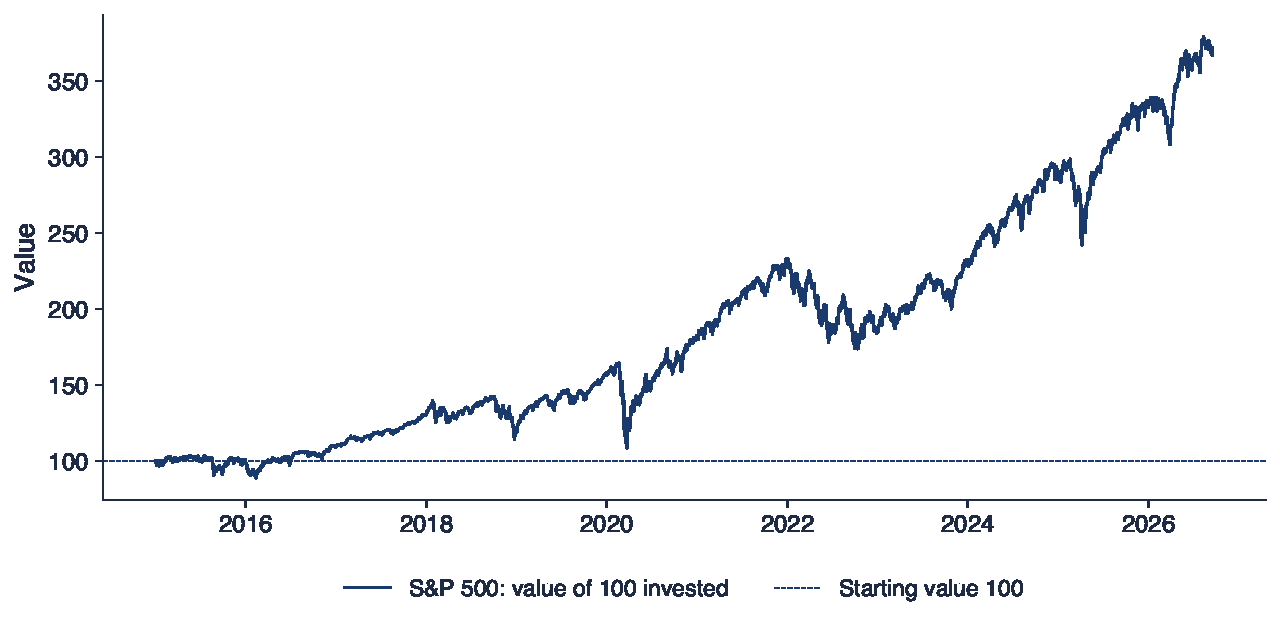
\includegraphics[width=0.94\textwidth,height=0.6\textheight,keepaspectratio]{ch0_sem_b1_growth.pdf}
\end{center}
\vspace{-2mm}
\begin{itemize}
    \item 100 de unități investite pe 2 ianuarie 2015 valorau 372 pe 18 septembrie 2026 (indice de preț, fără dividende)
\end{itemize}
\sfmquantlet{Ch_00}{SFM_ch0_seminar}
\end{frame}

\begin{frame}{B1 [Rezolvat]: Rezolvare (3/3) --- drawdown și interpretare}
\itemsize{\footnotesize}
\begin{columns}[T]
\begin{column}{0.55\textwidth}
\begin{center}
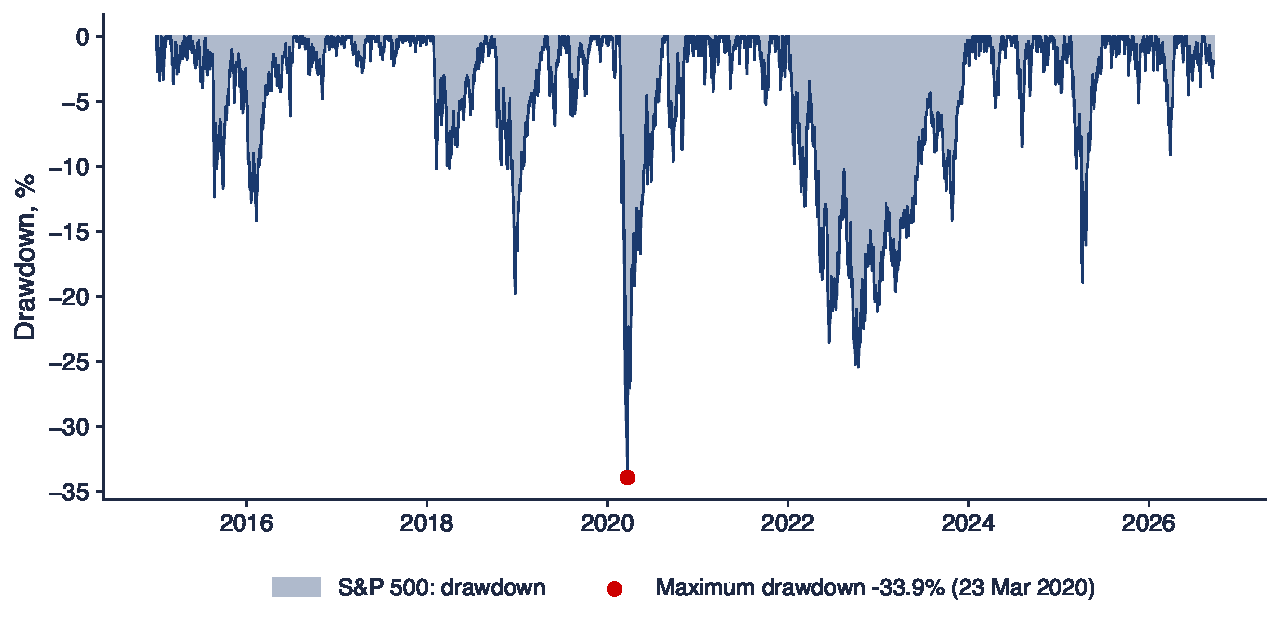
\includegraphics[width=0.94\textwidth,height=0.55\textheight,keepaspectratio]{ch0_sem_b1_drawdown.pdf}
\end{center}
\vspace{-2mm}

\end{column}
\begin{column}{0.42\textwidth}
\begin{itemize}
    \item \textbf{Drawdown-ul maxim}: -33{,}9\%, de la vîrful din 19 februarie 2020 la 23 martie 2020 (COVID-19)
    \item Al doilea episod ca adîncime: 2022, cînd au crescut dobînzile
    \item \textbf{Interpretare}
    \begin{itemize}
        \item un randament mediu anual bun (11{,}2\%) ascunde o scădere de o treime într-o singură lună
        \item raportați volatilitatea și drawdown-ul alături de medie
    \end{itemize}
\end{itemize}
\end{column}
\end{columns}
\sfmquantlet{Ch_00}{SFM_ch0_seminar}
\end{frame}

\begin{frame}{B2 [Rezolvat]: O cotație suspectă --- cerință}
\itemsize{\small}
\begin{itemize}
\item \textbf{Întrebarea}: este cea mai mare variație EUR/RON din seria de piață un preț real?
\item \textbf{Date}: seria EUR/RON de la EODHD (\texttt{eurron\_eodhd}) și cursul de referință BNR (\texttt{eurron}), 2015--2026
\item \textbf{Cerințe}
\begin{enumerate}
    \item Pentru fiecare zi, calculați diferența procentuală dintre cotația EODHD și cursul BNR din aceeași zi.
    \item Găsiți ziua cu cea mai mare diferență în valoare absolută și afișați cotațiile din ziua anterioară și din ziua următoare.
    \item Calculați randamentele logaritmice de intrare în acea zi și de ieșire din ea.
    \item Reprezentați grafic ambele serii în luna din jurul acelei zile.
\end{enumerate}
\item \textbf{Raportați}: data, cotația, cursul BNR, cele două randamente logaritmice și decizia voastră: preț real sau bad tick
\item Notebook: secțiunea B2
\end{itemize}
\end{frame}

\begin{frame}{B2 [Rezolvat]: Rezolvare (1/2) --- pas cu pas}
\itemsize{\small}
\begin{itemize}
    \item \textbf{Cea mai mare diferență}: 13 august 2025
    \begin{itemize}
        \item cotația EODHD 5{,}9065 față de cursul BNR 5{,}0633: o diferență de +16{,}7\%
        \item ziua anterioară (12 august 2025): 5{,}0636; ziua următoare (14 august 2025): 5{,}0629
    \end{itemize}
    \item \textbf{Două randamente logaritmice}
    \begin{itemize}
        \item la intrare: +15{,}4\%; la ieșire: -15{,}4\%
        \item pentru comparație, cea mai mare variație zilnică a cursului BNR din 2015 încoace este de 1{,}4\%
    \end{itemize}
    \item \textbf{Decizia}: un bad tick
    \begin{itemize}
        \item un salt de 15\% care se inversează complet a doua zi și lipsește din cursul oficial
        \item dacă ar rămîne în date, ar adăuga două dintre cele mai mari variații zilnice ale leului din ultimul deceniu
    \end{itemize}
    \item La curs și la seminar folosim pentru EUR/RON cursul de referință BNR
\end{itemize}
\sfmquantlet{Ch_00}{SFM_ch0_seminar}
\end{frame}

\begin{frame}{B2 [Rezolvat]: Rezolvare (2/2) --- grafic și interpretare}
\itemsize{\footnotesize}
\begin{center}
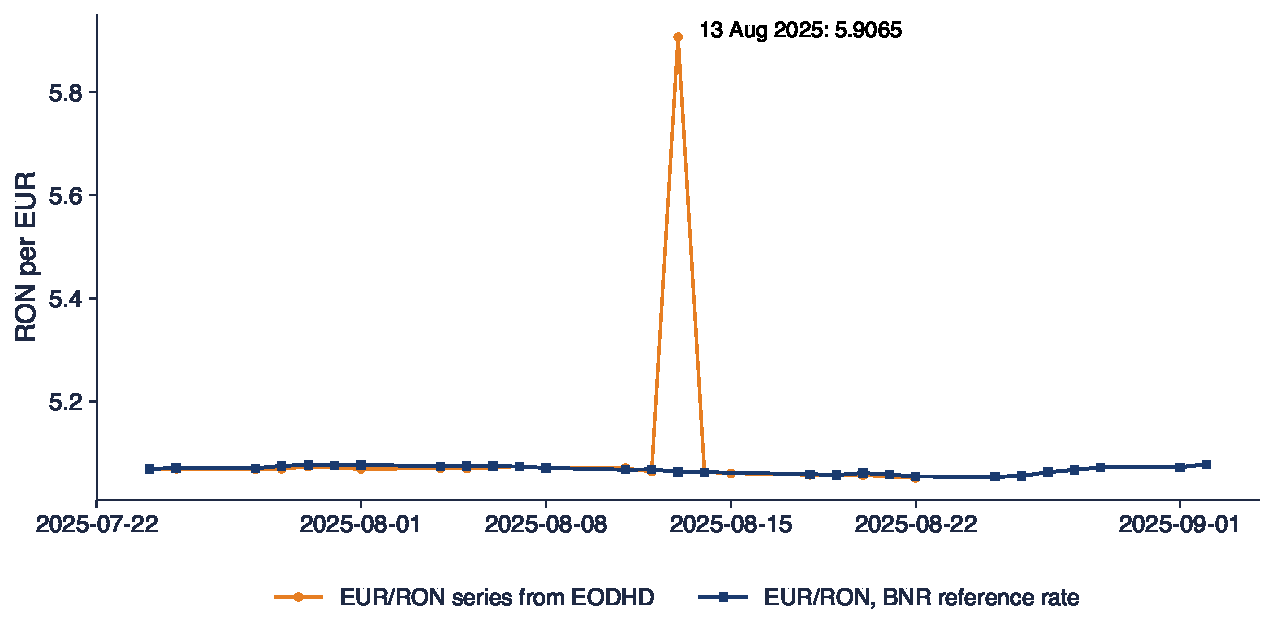
\includegraphics[width=0.94\textwidth,height=0.58\textheight,keepaspectratio]{ch0_sem_b2_eurron.pdf}
\end{center}
\vspace{-2mm}
\begin{itemize}
    \item O cotație departe de toate celelalte și de cursul oficial: priviți întotdeauna datele înainte de a calcula statistici
    \item Interpretare: o volatilitate calculată cu acest tick ar descrie o eroare, nu piața
\end{itemize}
\sfmquantlet{Ch_00}{SFM_ch0_seminar}
\end{frame}


%=============================================================================
\section{Rîndul vostru}
%=============================================================================

\begin{frame}{A4 [Propus]: Alte cifre --- cerință}
\itemsize{\small}
\begin{itemize}
\item \textbf{Întrebarea}: puteți repeta A1--A3 fără rezolvarea în față?
\item \textbf{Date}: o acțiune la $P_0 = 50$, $P_1 = 55$, $P_2 = 44$; un fond la 200, 180, 220, 165, 198, 230 în zilele 0--5; media zilnică $0{,}03\%$ și volatilitatea zilnică $1{,}5\%$
\item \textbf{Cerințe}
\begin{enumerate}
    \item Model: A1, A2 și A3 [Rezolvat].
    \item Calculați cele două randamente simple și cele două randamente logaritmice ale acțiunii, sumele lor și randamentele pe două zile.
    \item Calculați drawdown-ul fondului pentru fiecare zi și drawdown-ul lui maxim.
    \item Anualizați media și volatilitatea zilnice, cu $q = 252$.
\end{enumerate}
\item \textbf{Raportați}: cele două tabele, drawdown-ul maxim, cele două valori anuale și o propoziție care precizează ce sumă coincide cu randamentul pe două zile
\item Notebook: secțiunea A4
\end{itemize}
\end{frame}

\ifsolutions
\begin{frame}{A4: Rezolvare (profesor)}
\itemsize{\small}
\begin{itemize}
    \item \textbf{Acțiunea}
    \begin{itemize}
        \item $R_1 = +$10{,}00\%, $R_2 = $ -20{,}00\%; $r_1 = +$9{,}53\%, $r_2 = $ -22{,}31\%
        \item sume: -10{,}00\% (simple), -12{,}78\% (logaritmice); pe două zile: -12{,}00\% (simplu), -12{,}78\% (logaritmic)
        \item doar suma logaritmică este egală cu randamentul logaritmic pe două zile
    \end{itemize}
    \item \textbf{Fondul}
    \begin{itemize}
        \item $DD_t$: 0{,}0; -10{,}0; 0{,}0; -25{,}0; -10{,}0; 0{,}0 (\%)
        \item drawdown maxim -25{,}0\%, de la 220 (ziua 2) la 165 (ziua 3); vîrf nou în ziua 5
    \end{itemize}
    \item \textbf{Anualizarea}
    \begin{itemize}
        \item media $252 \times 0{,}03\% = $ 7{,}6\%; volatilitatea $\sqrt{252} \times 1{,}5\% = $ 23{,}8\%
    \end{itemize}
\end{itemize}
\end{frame}
\fi

\begin{frame}{B3 [Propus]: BET-TR, 2015--2026 --- cerință}
\itemsize{\small}
\begin{itemize}
\item \textbf{Întrebarea}: cum s-a comportat piața din România, cu dividende, față de S\&P 500?
\item \textbf{Date}: prețurile de închidere BET-TR de la 2 ianuarie 2015 (\texttt{load\_close('bettr')}) la 18 septembrie 2026
\item \textbf{Cerințe}
\begin{enumerate}
    \item Model: B1 [Rezolvat]; refolosiți codul și schimbați doar numele seriei.
    \item Calculați $q$, randamentul logaritmic mediu anualizat și volatilitatea anualizată.
    \item Calculați randamentul cumulat și drawdown-ul maxim, cu datele lui.
    \item Comparați fiecare cifră cu rezultatul S\&P 500 din B1.
\end{enumerate}
\item \textbf{Raportați}: un tabel cu două coloane (S\&P 500, BET-TR) și o propoziție: de ce comparația nu este pe deplin corectă?
\item Notebook: secțiunea B3
\end{itemize}
\end{frame}

\ifsolutions
\begin{frame}{B3: Rezolvare (profesor)}
\itemsize{\small}
\begin{columns}[T]
\begin{column}{0.45\textwidth}
\begin{center}
\footnotesize
\begin{tabular}{lrr}
\toprule
& S\&P 500 & BET-TR \\
\midrule
$q$ & 251{,}5 & 250{,}0 \\
media, \% pe an & 11{,}2 & 20{,}0 \\
volatilitatea, \% pe an & 17{,}7 & 15{,}5 \\
cumulat, \% & 271{,}7 & 938{,}5 \\
MDD, \% & -33{,}9 & -31{,}1 \\
\bottomrule
\end{tabular}
\end{center}

\end{column}
\begin{column}{0.52\textwidth}
\begin{itemize}
    \item BET-TR: drawdown maxim de la 23 ianuarie 2020 la 23 martie 2020
    \item \textbf{Interpretare}
    \begin{itemize}
        \item BET-TR: medie mai mare, volatilitate mai mică în această fereastră
        \item nu este pe deplin corectă: BET-TR include dividendele, indicele de preț S\&P 500 nu; monedele diferă (RON, USD)
    \end{itemize}
\end{itemize}
\end{column}
\end{columns}
\end{frame}
\fi

\begin{frame}{B4 [Propus]: Bitcoin: 365 sau 252 de zile? --- cerință}
\itemsize{\small}
\begin{itemize}
\item \textbf{Întrebarea}: cît de mare este eroarea dacă Bitcoin este anualizat ca un indice bursier?
\item \textbf{Date}: prețurile de închidere Bitcoin de la 2 ianuarie 2015 (\texttt{load\_close('btc')}) la 18 septembrie 2026
\item \textbf{Cerințe}
\begin{enumerate}
    \item Model: A2 și B1 [Rezolvat].
    \item Calculați din date numărul de randamente pe an $q$.
    \item Calculați volatilitatea anualizată cu $q = 365$, apoi cu $q = 252$.
    \item Calculați randamentul cumulat și drawdown-ul maxim, cu datele lui.
\end{enumerate}
\item \textbf{Raportați}: $q$, cele două volatilități și raportul lor, randamentul cumulat, drawdown-ul maxim și o propoziție care precizează care volatilitate este corectă
\item Notebook: secțiunea B4
\end{itemize}
\end{frame}

\ifsolutions
\begin{frame}{B4: Rezolvare (profesor)}
\itemsize{\small}
\begin{itemize}
    \item 4\,277 de randamente zilnice: $q = $ 365{,}3, deci 365 este corect
    \item \textbf{Volatilitatea}
    \begin{itemize}
        \item cu 365: 66{,}7\% pe an; cu 252: 55{,}4\% pe an
        \item raportul $\sqrt{365/252} = $ 1{,}20: folosirea lui 252 subestimează riscul cu aproximativ o șesime
    \end{itemize}
    \item \textbf{Randament și drawdown}
    \begin{itemize}
        \item media anuală 47{,}4\%; randament cumulat 25580{,}4\% (prețul $\times$257)
        \item drawdown maxim -83{,}4\%, de la 16 decembrie 2017 la 15 decembrie 2018
    \end{itemize}
    \item Interpretare: creșterea uriașă și pierderea de 83\% într-un an fac parte din aceeași serie
\end{itemize}
\end{frame}
\fi


%=============================================================================
\section{Partea C: critica unui răspuns generat de AI}
%=============================================================================

\begin{frame}[fragile]{C2 [Propus]: Critica unui răspuns generat de AI --- răspunsul}
\itemsize{\footnotesize}
\begin{itemize}
    \item \textbf{Cererea} trimisă unui asistent AI: „Din datele cursului, calculează volatilitatea anualizată și randamentul cumulat ale S\&P 500 și Bitcoin din 2 ianuarie 2015, din randamentele simple zilnice.”
\end{itemize}
\begin{lstlisting}
# read_market(symbol): the daily table of the course data
for name, sym in [('S&P 500', 'GSPC.INDX'), ('Bitcoin', 'BTC-USD.CC')]:
    p = read_market(sym)['close'].loc['2015-01-02':]   # closing prices
    R = p.pct_change().dropna()          # daily simple returns
    vol = R.std() * 252                  # annualised volatility
    cum = R.sum()                        # cumulative return
    print(name, round(100 * vol, 1), round(100 * cum, 1))
\end{lstlisting}
\begin{itemize}
    \item \textbf{Concluzia AI}: „Volatilitate: S\&P 500 280{,}3\%, Bitcoin 873{,}3\%. Randament cumulat: S\&P 500 149{,}6\%, Bitcoin 814{,}0\%. Bitcoin a cîștigat doar de aproximativ cinci ori mai mult decît S\&P 500.”
\end{itemize}
\end{frame}

\begin{frame}{C2 [Propus]: Critica unui răspuns generat de AI --- cerință}
\itemsize{\small}
\begin{itemize}
\item \textbf{Întrebarea}: puteți avea încredere într-un cod care rulează fără niciun mesaj de eroare?
\item \textbf{Date}: codul și concluzia de pe slide-ul anterior; definițiile din noțiunile de bază
\item \textbf{Cerințe}
\begin{enumerate}
    \item Model: A1, A2 și B1 [Rezolvat].
    \item Găsiți cele trei greșeli introduse intenționat în cod.
    \item Pentru fiecare greșeală, precizați cum ați detecta-o: o verificare a rezultatului, noțiunile de bază sau un exercițiu rezolvat.
    \item Scrieți codul corectat și raportați volatilitatea și randamentul cumulat corectate pentru ambele active.
    \item Precizați dacă mai rămîne valabilă concluzia „Bitcoin a cîștigat doar de aproximativ cinci ori mai mult”.
\end{enumerate}
\item \textbf{Raportați}: un tabel cu rezultatele AI și cele corectate și cîte o linie pentru fiecare greșeală, în formatul: cerere, răspuns, greșeală, cum a fost găsită, corectare
\item Notebook: secțiunea C2
\end{itemize}
\end{frame}

\ifsolutions
\begin{frame}{C2: Rezolvare (profesor)}
\itemsize{\footnotesize}
\begin{columns}[T]
\begin{column}{0.50\textwidth}
\begin{itemize}
    \item \textbf{Greșeala 1}: \texttt{R.std() * 252}; volatilitatea se anualizează cu factorul $\sqrt{252}$
    \begin{itemize}
        \item detectare: o volatilitate de 280{,}3\% pe an pentru un indice bursier este imposibilă (A2)
    \end{itemize}
    \item \textbf{Greșeala 2}: 252 de zile pentru Bitcoin, care se tranzacționează în fiecare zi
    \begin{itemize}
        \item detectare: numărați observațiile pe an (365{,}3)
    \end{itemize}
    \item \textbf{Greșeala 3}: \texttt{R.sum()} nu este randamentul cumulat; randamentele simple se compun
    \begin{itemize}
        \item detectare: comparați cu $P_T/P_0 - 1$ (A1, B1)
    \end{itemize}
\end{itemize}
\end{column}
\begin{column}{0.47\textwidth}
\begin{center}
\footnotesize
\begin{tabular}{lrr}
\toprule
& Vol. \% & Cumulat \% \\
\midrule
S\&P 500, AI & 280{,}3 & 149{,}6 \\
S\&P 500, corectat & 17{,}7 & 271{,}7 \\
Bitcoin, AI & 873{,}3 & 814{,}0 \\
Bitcoin, corectat & 66{,}2 & 25580{,}4 \\
\bottomrule
\end{tabular}
\end{center}
\begin{itemize}
    \item Corectat: \texttt{R.std() * np.sqrt(q)} cu $q$ = 252 sau 365 și \texttt{p.iloc[-1] / p.iloc[0] - 1}
    \item Concluzia nu se susține: Bitcoin a cîștigat de aproximativ 94{,}1 ori mai mult decît S\&P 500, nu de 5{,}4 ori, cu o volatilitate de 3{,}7 ori mai mare
\end{itemize}
\end{column}
\end{columns}
\end{frame}
\fi


%=============================================================================
\section{Încheiere}
%=============================================================================

\begin{frame}{Exerciții pentru acasă}
\itemsize{\small}
\begin{itemize}
    \item \textbf{Terminați exercițiile propuse}: A4, B3, B4 și C2
    \begin{itemize}
        \item fiecare indică exercițiul rezolvat care servește drept model
        \item rezolvările se discută la seminarul următor
    \end{itemize}
    \item \textbf{Încercați încă o serie}
    \begin{itemize}
        \item repetați B1 pentru DAX (\texttt{dax}) sau pentru aur (\texttt{gold}) și comparați volatilitățile anuale
    \end{itemize}
    \item \textbf{Rezolvați quiz-ul \sfmchlink{https://danpele.github.io/SFM/RO/Cursuri/capitol0_introducere.pdf}{Capitolului 0}} pe site-ul cursului: 20 de întrebări, cu explicație pentru fiecare răspuns
    \item Temele nu se notează: sînt pregătire pentru examen și pentru proiect
\end{itemize}
\end{frame}

\begin{frame}{Recapitulare; urmează cursul din \sfmchlinkt{https://danpele.github.io/SFM/RO/Cursuri/capitol0_introducere.pdf}{Capitolul 0}}
\itemsize{\small}
\begin{columns}[T]
\begin{column}{0.52\textwidth}
\begin{itemize}
    \item \textbf{Azi}
    \begin{itemize}
        \item randamentele simple se compun, cele logaritmice se adună
        \item anualizăm media cu $q$ și volatilitatea cu $\sqrt{q}$; $q = 365$ pentru Bitcoin
        \item drawdown-ul maxim este cea mai mare pierdere față de un vîrf
        \item priviți întîi datele: un singur bad tick poate domina o statistică
        \item codul generat de AI poate rula și totuși să fie greșit
    \end{itemize}
\end{itemize}
\end{column}
\begin{column}{0.45\textwidth}
\begin{itemize}
    \item \textbf{La curs}
    \begin{itemize}
        \item Cum este organizat și evaluat cursul?
        \item Cum arată piețele din 2026 în date?
        \item Cum au evoluat bursele, crahurile și modelele?
        \item De ce randamentele zilnice nu urmează distribuția Normală?
    \end{itemize}
\end{itemize}
\end{column}
\end{columns}
\end{frame}

\end{document}
